\documentclass{article}
\usepackage{physics}
\usepackage{graphicx}
\usepackage{caption}
\usepackage{amsmath}
\usepackage{bm}
\usepackage{framed}
\usepackage{authblk}
\usepackage{empheq}
\usepackage{amsfonts}
\usepackage{esint}
\usepackage[makeroom]{cancel}
\usepackage{dsfont}
\usepackage{centernot}
\usepackage{mathtools}
\usepackage{bigints}
\usepackage{amsthm}
\theoremstyle{definition}
\newtheorem{defn}{Definition}[section]
\newtheorem{prop}{Proposition}[section]
\newtheorem{rmk}{Remark}[section]
\newtheorem{thm}{Theorem}[section]
\newtheorem{exmp}{Example}[section]
\newtheorem{prob}{Problem}[section]
\newtheorem{sln}{Solution}[section]
\newtheorem*{prob*}{Problem}
\newtheorem{exer}{Exercise}[section]
\newtheorem*{exer*}{Exercise}
\newtheorem*{sln*}{Solution}
\usepackage{empheq}
\usepackage{tensor}
\usepackage{xcolor}
%\definecolor{colby}{rgb}{0.0, 0.0, 0.5}
\definecolor{MIT}{RGB}{163, 31, 52}
\usepackage[pdftex]{hyperref}
%\hypersetup{colorlinks,urlcolor=colby}
\hypersetup{colorlinks,linkcolor={MIT},citecolor={MIT},urlcolor={MIT}}  
\usepackage[left=1in,right=1in,top=1in,bottom=1in]{geometry}

\usepackage{newpxtext,newpxmath}
\newcommand*\widefbox[1]{\fbox{\hspace{2em}#1\hspace{2em}}}

\newcommand{\p}{\partial}
\newcommand{\R}{\mathbb{R}}
\newcommand{\C}{\mathbb{C}}
\newcommand{\lag}{\mathcal{L}}
\newcommand{\nn}{\nonumber}
\newcommand{\ham}{\mathcal{H}}
\newcommand{\M}{\mathcal{M}}
\newcommand{\I}{\mathcal{I}}
\newcommand{\K}{\mathcal{K}}
\newcommand{\F}{\mathcal{F}}
\newcommand{\w}{\omega}
\newcommand{\lam}{\lambda}
\newcommand{\al}{\alpha}
\newcommand{\be}{\beta}
\newcommand{\x}{\xi}

\newcommand{\G}{\mathcal{G}}

\newcommand{\f}[2]{\frac{#1}{#2}}

\newcommand{\ift}{\infty}

\newcommand{\lp}{\left(}
\newcommand{\rp}{\right)}

\newcommand{\lb}{\left[}
\newcommand{\rb}{\right]}

\newcommand{\lc}{\left\{}
\newcommand{\rc}{\right\}}


\newcommand{\V}{\mathbf{V}}
\newcommand{\U}{\mathcal{U}}
\newcommand{\Id}{\mathcal{I}}
\newcommand{\D}{\mathcal{D}}
\newcommand{\Z}{\mathcal{Z}}

%\setcounter{chapter}{-1}


\usepackage{enumitem}



\usepackage{subfig}
\usepackage{listings}
\captionsetup[lstlisting]{margin=0cm,format=hang,font=small,format=plain,labelfont={bf,up},textfont={it}}
\renewcommand*{\lstlistingname}{Code \textcolor{violet}{\textsl{Mathematica}}}
\definecolor{gris245}{RGB}{245,245,245}
\definecolor{olive}{RGB}{50,140,50}
\definecolor{brun}{RGB}{175,100,80}

%\hypersetup{colorlinks,urlcolor=colby}
\lstset{
	tabsize=4,
	frame=single,
	language=mathematica,
	basicstyle=\scriptsize\ttfamily,
	keywordstyle=\color{black},
	backgroundcolor=\color{gris245},
	commentstyle=\color{gray},
	showstringspaces=false,
	emph={
		r1,
		r2,
		epsilon,epsilon_,
		Newton,Newton_
	},emphstyle={\color{olive}},
	emph={[2]
		L,
		CouleurCourbe,
		PotentielEffectif,
		IdCourbe,
		Courbe
	},emphstyle={[2]\color{blue}},
	emph={[3]r,r_,n,n_},emphstyle={[3]\color{magenta}}
}






\begin{document}
	
\begin{framed}
	\noindent Name: \textbf{Huan Q. Bui}\\
	Course: \textbf{8.309 - Classical Mechanics III}\\
	Problem set: \textbf{\#8}
\end{framed}

\noindent \textbf{1. Flow Geometries.} For an ideal fluid, $\vec{v} \cdot \hat{n} = 0$ where $\hat{n}$ is the normal to the surface. Thus, we may look for $\hat{n}$ by computing $\grad \phi$ and solve for $(\grad \phi)\cdot \hat{n} = 0$
 
\begin{enumerate}[label=(\alph*)]
	\item Set $C=1$, so that we find that $\vec{v} = \grad_\text{cyl} \phi = \grad_\text{cyl} r^2\cos(2\theta) = (2r\cos2\theta, -2r\sin2\theta,0)$. From here we find that 
	\begin{align*}
	\hat{n} = (\sin 2 \theta, \cos 2 \theta) = \sin 2 \theta \hat{r} + \cos 2 \theta \hat{\theta}
	\end{align*}
	where we have ignored the $z$-component. By the form of $\vec{v}$, we can see that there is one stagnation point at $r=0$, which is the origin. 

	\begin{figure}[!htb]
		\centering
		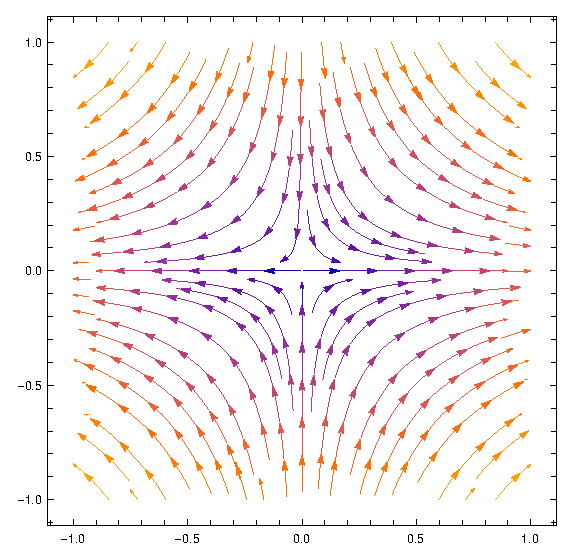
\includegraphics[width=0.3\textwidth]{1a.eps}
		\caption{Generated using Mathematica's \texttt{StreamPlot}}
	\end{figure}
	
	Mathematica code:
	\begin{lstlisting}
	In[4]:= Grad[r^2*Cos[2*\[Theta]], {r, \[Theta], z}, "Cylindrical"]
	
	Out[4]= {2 r Cos[2 \[Theta]], -2 r Sin[2 \[Theta]], 0}
	
	In[55]:= StreamPlot[
	Evaluate[TransformedField[
	"Polar" -> 
	"Cartesian", {2*r*Cos[2 \[Theta]], -2*r* 
	Sin[2 \[Theta]]}, {r, \[Theta]} -> {x, y}]], {x, -1, 1}, {y, -1, 
	1}]
	\end{lstlisting}
	
	
	
	
	
	\item Set $C=1$, so that we find that $\vec{v} = \grad_\text{cyl} \phi = \grad_\text{cyl} r^4 \cos(4\theta) = (4r^3\cos 4\theta, -4r^3 \sin4 \theta,0)$. From here we find that 
	\begin{align*}
	\hat{n} = (\sin 4 \theta, \cos 4 \theta) = \sin 4 \theta \hat{r} + \cos 4 \theta \hat{\theta}
	\end{align*}
	where we have ignored the $z$-component. By the form of $\vec{v}$, we can see that there is one stagnation point at $r=0$, which is the origin. \\
	
	\begin{figure}[!htb]
		\centering
		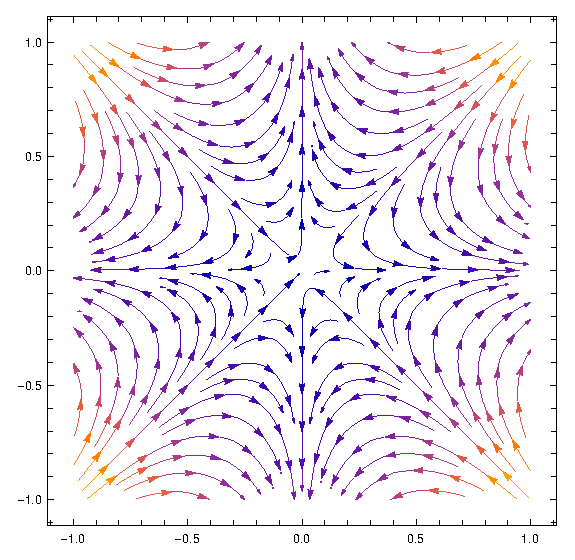
\includegraphics[width=0.3\textwidth]{1b.eps}
		\caption{Generated using Mathematica's \texttt{StreamPlot}}
	\end{figure}
	
	Mathematica code:
	\begin{lstlisting}
	In[6]:= Grad[r^4*Cos[4*\[Theta]], {r, \[Theta], z}, "Cylindrical"]
	
	Out[6]= {4 r^3 Cos[4 \[Theta]], -4 r^3 Sin[4 \[Theta]], 0}
	
	In[56]:= StreamPlot[
	Evaluate[TransformedField[
	"Polar" -> 
	"Cartesian", {4 r^3 Cos[4 \[Theta]], -4 r^3 Sin[
	4 \[Theta]]}, {r, \[Theta]} -> {x, y}]], {x, -1, 1}, {y, -1, 1}]
	\end{lstlisting}
	
	\item \textbf{Optional for me (8.309):} Set $C=1$, so that we find that $\vec{v} = \grad_\text{cyl} \phi = \grad_\text{cyl} r^{2/3} \cos(2\theta/3) = ((2/3)r^{-1/3}\cos (2\theta/3), -(2/3)r^{-1/3} \sin (2 \theta/3),0)$. From here we find that 
	\begin{align*}
	\hat{n} = (\sin (2 \theta/3), \cos (2 \theta/3)) = \sin (2 \theta/3) \hat{r} + \cos (2 \theta/3) \hat{\theta}
	\end{align*}
	where we have ignored the $z$-component. By the form of $\vec{v}$, we can see that there is no stagnation point at any finite $r$. \\
	
	\begin{figure}[!htb]
		\centering
		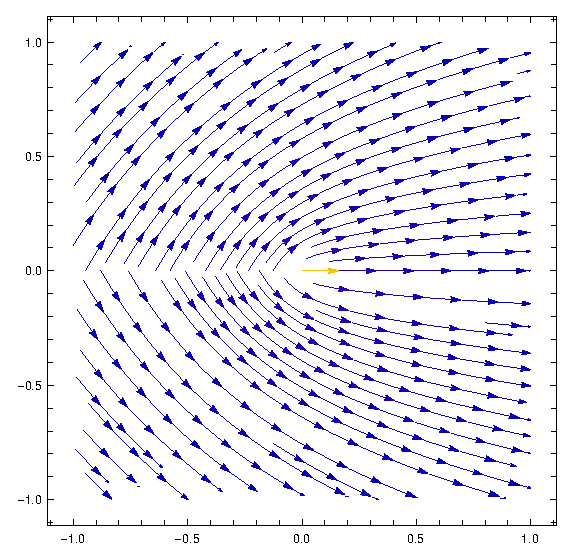
\includegraphics[width=0.3\textwidth]{1c.eps}
		\caption{Generated using Mathematica's \texttt{StreamPlot}}
	\end{figure}
	
	Mathematica code:
	\begin{lstlisting}
	In[8]:= Grad[
	r^(2/3)*Cos[2*\[Theta]/3], {r, \[Theta], z}, "Cylindrical"]
	
	Out[8]= {(2 Cos[(2 \[Theta])/3])/(
	3 r^(1/3)), -((2 Sin[(2 \[Theta])/3])/(3 r^(1/3))), 0}
	
	In[57]:= StreamPlot[
	Evaluate[TransformedField[
	"Polar" -> "Cartesian", {(2 Cos[(2 \[Theta])/3])/(
	3 r^(1/3)), -((2 Sin[(2 \[Theta])/3])/(
	3 r^(1/3)))}, {r, \[Theta]} -> {x, y}]], {x, -1, 1}, {y, -1, 1}]
	\end{lstlisting}
	
	
	
\end{enumerate}

\noindent \textbf{2. The Stream Function}

\begin{enumerate}[label=(\alph*)]
	\item Streamlines are lines that are everwhere tangent to the instantaneous velocity:
	\begin{align*}
	\f{d}{dt}\mathbf{x}(s) \times \mathbf{v} =0 \implies \f{dy}{dx} = \f{v_y}{v_x}
	\end{align*}
	Lines of constant $\psi$ are characterized by $d\psi = 0$, which means 
	\begin{align*}
	0 = d\psi = \f{\p \psi}{\p x} \, dx + \f{\p \psi}{\p y} \, dy \implies -v_y \,dx + v_x\,dy = 0 \implies \f{dy}{dx} = \f{v_y}{v_x}
	\end{align*}
	same as above. We therefore conclude that streamlines are lines of constant $\psi$. 
	
	
	\item If $\curl \mathbf{v} = 0$, then 
	\begin{align*}
	0 = \f{\p v_y }{\p x} - \f{\p v_x}{\p y} = -\f{\p^2 \psi }{\p x^2} - \f{\p^2 \psi }{\p y^2} \implies  \nabla^2 \psi = 0
	\end{align*}
	which means $\psi$ solves Laplace's equation. \\
	
	
	
	
	
	Working in Cartesian coordinates, we have
	\begin{align*}
	&v_x = \f{\p \phi}{\p x} = \f{\p \psi}{\p y} \\
	&v_y = \f{\p \phi}{\p y} = -\f{\p \psi}{\p x}
	\end{align*}
	In polar coordinates we have
	\begin{align*}
	&v_r = \f{\p \phi}{\p r} = \f{1}{r}\f{\p \psi}{\p \theta} = \sqrt{r} \cos\lp \f{3\theta}{2} \rp\\
	&v_\theta = \f{1}{r}\f{\p \phi}{\p \theta} = -\f{\p \psi}{\p r} = -\sqrt{r}\sin\lp \f{3\theta}{2} \rp
	\end{align*}
	Mathematica code:
	\begin{lstlisting}
	In[61]:= \[Psi] = (2/3)*r^(3/2)*Sin[3 \[Theta]/2];
	
	In[62]:= ur = (1/r)*D[\[Psi], \[Theta]]
	
	Out[62]= Sqrt[r] Cos[(3 \[Theta])/2]
	
	In[63]:= u\[Theta] = -D[\[Psi], r]
	
	Out[63]= -Sqrt[r] Sin[(3 \[Theta])/2]
	\end{lstlisting}
	So, by inspection we get
	\begin{align*}
	\boxed{\phi = \f{2}{3}r^{3/2}\cos\lp \f{3\theta}{2} \rp}
	\end{align*}
	To check, we can compute the gradient of $\phi$ to find 
	\begin{align*}
	\grad \phi = \lc \sqrt{r} \cos\lp \f{3\theta}{2} \rp, -\sqrt{r}\sin\lp \f{3\theta}{2} \rp ,0 \rc \quad\quad \quad \checkmark
	\end{align*}
	Check in Mathematica:
	\begin{lstlisting}
	In[64]:= Grad[(2/3) r^(3/2)*Cos[3*\[Theta]/2], {r, \[Theta], 
	z}, "Cylindrical"]
	
	Out[64]= {Sqrt[r] Cos[(3 \[Theta])/2], -Sqrt[r] Sin[(3 \[Theta])/2],
	0}
	\end{lstlisting}
	
	
	

 
\end{enumerate}

\newpage


\noindent \textbf{3. Ideal Fluid Flow around a Cylinder.} 

\begin{enumerate}[label=(\alph*)]
	\item Let the flow potential $\phi$ be given. It must satisfy the Laplace's equation in polar coordinates:
	\begin{align*}
	\nabla^2 \phi = \f{1}{r}\f{\p}{\p r}\lp r\f{\p \phi}{\p r} \rp + \f{1}{r^2}\f{\p^2 \phi}{\p \theta^2} = 0. 
	\end{align*}
	By separation of variables, we may write
	\begin{align*}
	\phi(r,\theta) = R(r)\Theta(\theta)
	\end{align*}
	where
	\begin{align*}
 	\f{r}{R}\f{\p}{\p r}\lp r\f{\p R}{\p r} \rp = -\f{1}{\Theta}\f{\p^2 \Theta}{\p \theta^2} = \lambda^2
	\end{align*}
	where $\lambda > 0$ is some constant. Solving for $\Theta$ gives
	\begin{align*}
	\Theta(\theta) = A\cos \lambda \theta + B \sin\lambda \theta.
	\end{align*}
	On the other hand solving for $R(r)$ gives
	\begin{align*}
	R(r) = Cr^{-\lambda} + D r^{\lambda}.
	\end{align*}
	The general solution is 
	\begin{align*}
	\phi(r,\theta) &= \sum_{\lambda = 1}^\infty (C_\lambda r^{-\lambda} + D_\lambda r^{\lambda}) (A_\lambda\cos\lambda\theta + B_\lambda\sin\lambda\theta) \\ 
	&= \lp \f{C_1}{r} + D_1r \rp(A_1 \cos\theta + B_1 \sin\theta) + \sum_{\lambda = 2}^\infty (C_\lambda r^{-\lambda} + D_\lambda r^{\lambda}) (A_\lambda\cos\lambda\theta + B_\lambda\sin\lambda\theta).
	\end{align*}
	Now we apply the boundary conditions by computing the velocity field:
	\begin{align*}
	\mathbf{v} = \grad \phi = \f{\p \phi}{\p r} \hat{r} + \f{1}{r}\f{\p \phi}{\p \theta} \hat{\theta}.
	\end{align*}
	We compute:
	\begin{align*}
	\f{\p \phi}{\p r} &= \lp \f{-C_1}{r^2} + D_1 \rp 
	(A_1 \cos\theta + B_1 \sin\theta) 
	+ \sum_{\lambda = 2}^\infty (-\lambda C_\lambda r^{-\lambda-1} + \lambda D_\lambda r^{\lambda-1}) (A_\lambda\cos\lambda\theta + B_\lambda\sin\lambda\theta)\\
	\f{1}{r}\f{\p \phi}{\p \theta} &=  \f{1}{r}\lb \lp \f{C_1}{r} + D_1r \rp(A_1 \cos\theta + B_1 \sin\theta) + \sum_{\lambda = 2}^\infty (C_\lambda r^{-\lambda} + D_\lambda r^{\lambda}) (A_\lambda\cos\lambda\theta + B_\lambda\sin\lambda\theta) \rb \\
	&= \f{1}{r}\lb \lp \f{C_1}{r} + D_1r \rp
	(-A_1 \cos\theta + B_1 \sin\theta) + \sum_{\lambda = 2}^\infty (C_\lambda r^{-\lambda} + D_\lambda r^{\lambda}) (-\lambda A_\lambda\cos\lambda\theta + \lambda B_\lambda\sin\lambda\theta) \rb.
	\end{align*}
	When $r\to \infty$, $\mathbf{v} = u \hat{x} \implies \f{\p \phi}{\p x}\big\vert_\infty = u \implies \phi(r,\theta)\big\vert_\infty = u r \cos\theta$, since $x = r\cos\theta$. With this, we may ignore all terms with $\lambda \geq 2$ and require that
	\begin{align*}
	B_1 = 0 \quad \text{and} \quad D_1 A_1 = u.	
	\end{align*}
	We also require that at $r=R$, $\mathbf{v}_r$ vanishes since no fluid could flow through the cylidner surface, which means that $C_1 A_1 = D_1 A_1 R^2 = uR^2$. So, the solution is 
	\begin{align*}
	\boxed{\phi(r,\theta) = u r \lp 1 + \f{R^2}{r^2} \rp\cos\theta}
	\end{align*}
	From here, the velocity field is 
	\begin{align*}
	\boxed{\mathbf{v} = u\lp 1 - \f{R^2}{r^2} \rp \cos\theta \hat{r} 
		- u \lp 1 + \f{R^2}{r^2}\rp\sin\theta \hat{\theta}}
	\end{align*}
	Mathematica code:
	\begin{lstlisting}
	In[110]:= 
	Grad[u*r*(1 + R^2/r^2)*Cos[\[Theta]], {r, \[Theta], z}, 
	"Cylindrical"] // FullSimplify
	
	Out[110]= {(1 - R^2/
	r^2) u Cos[\[Theta]], -((1 + R^2/r^2) u Sin[\[Theta]]), 0}
	\end{lstlisting}
	
	
	
	\item Since the fluid is ideal, incompressible, and irrotational, we may use Bernoulli's equation to obtain the pressure exerted on the cylinder: 
	\begin{align*}
	\lp \mathcal{P} + \f{1}{2}\rho v^2 \rp\bigg\vert_{r= R} = \lp \mathcal{P} + \f{1}{2}\rho v^2  \rp_{r=\infty} \implies \mathcal{P}_R
	& = \mathcal{P}_\infty + \f{\rho}{2}(v^2_\infty - {v^2_R})\\ 
	&= \mathcal{P}_\infty + \f{\rho}{2}(u^2 - 4u^2\sin^2\theta) \\
	&= \boxed{\mathcal{P}_\infty + \f{u^2\rho}{2}(2\cos 2 \theta - 1)} \\
	\end{align*}
	where we have used 
	\begin{align*}
	v_R^2 = v_r(R)^2 + v_\theta(R)^2.
	\end{align*}
	Mathematica code:
	\begin{lstlisting}
	(*velocity components*)
	In[108]:= vr = D[u*r*(1 + R^2/r^2)*Cos[\[Theta]], r] // FullSimplify
	
	Out[108]= (1 - R^2/r^2) u Cos[\[Theta]]
	
	In[109]:= v\[Theta] = (1/r)*
	D[u*r*(1 + R^2/r^2)*Cos[\[Theta]], \[Theta]] // FullSimplify
	
	Out[109]= -((1 + R^2/r^2) u Sin[\[Theta]])
	
	(*compute v^2*)
	In[111]:= vr^2 + v\[Theta]^2 /. {r -> R} // FullSimplify
	
	Out[111]= 4 u^2 Sin[\[Theta]]^2
	
	(*simplify*)
	In[112]:= u^2 - 4 u^2 Sin[\[Theta]]^2 // FullSimplify
	
	Out[112]= u^2 (-1 + 2 Cos[2 \[Theta]])
	\end{lstlisting}
	
	\item Let a streamline be given. Let it have the form $y(x)$ which satisfies the differential equation:
	\begin{align*}
	\f{dy}{dx} = \f{v_y}{v_x}
	\end{align*}
	To check that the solution 
	\begin{align*}
	x^2 + y^2 = \f{R^2}{1 - K/y}
	\end{align*}
	satisfies the equation above, we may compute $v_y/v_x$ from the derived velocity field, and compare it to $dy/dx$ which we will obtain from the solution. Using Mathematica, we can transform the velocity field from polar/cylindrical coordinates into Cartesian coordinates:
	\begin{align*}
	\mathbf{v}(r,\theta) \to \mathbf{v}(x,y) = \lb u + \f{R^2 u (-x^2 + y^2)}{(x^2 + y^2 )^2} \rb \hat{x} + \lb \f{-2R^2 u xy}{(x^2 + y^2)^2} \rb  \hat{y}
	\end{align*}	
	from which we can calculate:
	\begin{align*}
	\f{v_y}{v_x} = \f{\mp 2(K-y)^2 \sqrt{y(-y+\f{R^2}{-K+y})}}{2 K^2 y + 2y^3 + K(R^2 - 4y^2)} = \f{\mp 2(K-y)^2 \sqrt{y(-y+\f{R^2}{-K+y})}}{KR^2 + 2y(K-y)^2}
	\end{align*}
	where we have used
	\begin{align*}
	x = \pm \sqrt {\f{R^2}{1-K/y} - y^2}
	\end{align*}
	Now, we will calculate $\f{dy}{dx}$ using  $dy/dx = (dx/dy)^{-1}$. 
	\begin{align*}
	\f{dy}{dx} = \lb \pm \f{d}{dy}  \sqrt {\f{R^2}{1-K/y} - y^2} \rb^{-1} = \mp \f{2\sqrt{y(-y + \f{R^2}{-K+y})}}{\f{KR^2}{(K-y)^2} + 2y} =  \f{\mp 2(K-y)^2 \sqrt{y(-y + \f{R^2}{-K+y})}}{KR^2  + 2y(K-y)^2} = \f{v_y}{v_x} \quad \checkmark
	\end{align*}
	We see that the differential equation is satisfied, as desired. \\
	
	
	Mathematica code:
	\begin{lstlisting}
	(*Transform to Cartesian*)
	In[118]:= vxy = 
	TransformedField[
	"Polar" -> 
	"Cartesian", {(1 - R^2/
	r^2) u Cos[\[Theta]], -((1 + R^2/
	r^2) u Sin[\[Theta]])}, {r, \[Theta]} -> {x, y}] // 
	FullSimplify
	
	Out[118]= {u + (R^2 u (-x^2 + y^2))/(x^2 + y^2)^2, -((
	2 R^2 u x y)/(x^2 + y^2)^2)}
	
	(*Take ratio vy/vx*)
	In[135]:= 
	vxy[[2]]/vxy[[1]] /. {x -> Sqrt[R^2/(1 - K/y) - y^2]} // FullSimplify
	
	Out[135]= -((2 (K - y)^2 Sqrt[y (-y + R^2/(-K + y))])/(
	2 K^2 y + 2 y^3 + K (R^2 - 4 y^2)))
	
	(*Compute dy/dx = (dx/dy)^{-1}*)
	In[139]:= 1/D[Sqrt[R^2/(1 - K/y) - y^2], y] // FullSimplify
	
	Out[139]= -((2 Sqrt[y (-y + R^2/(-K + y))])/((K R^2)/(K - y)^2 + 2 y))
	\end{lstlisting}
\end{enumerate}




\noindent \textbf{4. A Spherical Sound Wave}

\begin{enumerate}[label=(\alph*)]
	\item The sound wave equation is 
	\begin{align*}
	\f{\p^2 p}{\p t^2} - c_s^2 \laplacian p = 0.
	\end{align*}
	From 
	\begin{align*}
	p = \f{1}{r}f(r - c_s t),
	\end{align*}
	we may compute in spherical coordinates
	\begin{align*}
	\f{\p^2 p }{\p t^2} - c_s^2 \laplacian p  
	&= \f{1}{r} c_s^2 f''(r-c_s t) - c_s^2 \f{1}{r^2} \f{\p }{\p r}\lb r^2 \f{\p p }{\p r}  \rb\\ 
	&=  \f{1}{r} c_s^2 f''(r-c_s t) - c_s^2 \f{1}{r^2} \f{\p }{\p r} \lb -f(r-c_s t) + r f'(r-c_s t) \rb \\
	&=  \f{1}{r} c_s^2 f''(r-c_s t) - c_s^2 \f{1}{r^2} \lb -f'(r-c_s t) + f'(r-c_s t) + r f''(r-c_s t) \rb \\
	&=  \f{1}{r} c_s^2 f''(r-c_s t) - c_s^2 \f{r}{r^2} f''(r-c_s t) \\
	&= 0 \quad\quad \checkmark
	\end{align*}
	
	\item To get the velocity field, we may start with
	\begin{align*}
	\f{\p \mathbf{v}}{\p t} &= -\f{\grad p}{\rho_0} \\
	&= -\f{1}{\rho_0} \f{\p p}{\p r} \hat{r}\\
	&= -\f{1}{\rho_0} \lb -\f{1}{r^2}f(r-c_s t) + \f{1}{r} f' (r-c_s t)  \rb \hat{r}\\
	&= \lb \f{1}{\rho_0 r^2} f(r-c_s t) - \f{1}{\rho_0 r} f' (r-c_s t) \rb \hat{r}
	\end{align*}
	from which we get
	\begin{align*}
	\mathbf{v} = \lb \f{1}{\rho_0 r^2} \int f(r-c_s t)\,dt - \f{1}{\rho_0 r }\int f' (r-c_s t) \,dt \rb \hat{r}.
	\end{align*}
	Let $x = r- c_s t$, then we may rewrite the integrals to get
	\begin{align*}
	\mathbf{v} = \lb \f{1}{\rho_0 r^2} \int f(r-c_s t)\,dt - \f{1}{\rho_0 r }\int f' (r-c_s t) \,dt \rb \hat{r}.
	\end{align*}
	\textbf{\textcolor{blue}{I'm not sure how to group the time dependence as suggested by the question (and I might do it incorrectly) so I'll just leave my answer in this explicit form.}}
	
	
	\item Here we verify that $\mathbf{v}$ satisfies the wave equation. The LHS is 
	\begin{align*}
	\f{\p^2 \mathbf{v}}{\p t^2} = \f{-c_s}{\rho_0 r^2} f'(r- c_s t) +  \f{c_s}{\rho_0 r} f''(r-c_s t)
	\end{align*}
	while the RHS is 
	\begin{align*}
	c_s^2 \nabla^2 \mathbf{v} &= 
	c_s^2  \nabla^2 \lb \f{1}{\rho_0 r^2} \int f(r-c_s t)\,dt - \f{1}{\rho_0 r }\int f' (r-c_s t) \,dt \rb \hat{r} \\
	&\quad\quad - \f{2c_s^2}{r^2}\lb \f{1}{\rho_0 r^2} \int f(r-c_s t)\,dt - \f{1}{\rho_0 r }\int f' (r-c_s t) \,dt \rb \hat{r} \\
	&= \f{c_s }{\rho_0  r^2}\lb -f'(r-c_s t) + rf''(r - c_s t)\rb \\
	&= \f{-c_s}{\rho_0 r^2} f'(r- c_s t) +  \f{c_s}{\rho_0 r} f''(r-c_s t) \\
	&= \f{\p ^2 \mathbf{v}}{\p t^2}. \quad\quad \checkmark
	\end{align*}
	So, the wave equation for the velocity field is satisfied. \\
	
	
	Mathematica code for the simplification of the RHS:
	\begin{lstlisting}
	In[69]:= F = (1/(\[Rho]*r^2)*
	Integrate[f[r - cs*t], t]) - (1/(\[Rho]*r))*
	Integrate[f'[r - cs*t], t];
	
	In[72]:= cs^2*(1/r^2)*D[r^2*D[F, r], r] - 2*cs^2/r^2*F // FullSimplify
	
	Out[72]= (cs (-Derivative[1][f][r - cs t] + 
	r (f^\[Prime]\[Prime])[r - cs t]))/(r^2 \[Rho])
	\end{lstlisting}
	
\end{enumerate}



\noindent \textbf{5. Viscous Fluid Velocity between Coaxial Cylinders.}  This is analogous to flow between two relatively moving infinite sheets. The Navier-Stokes equation is 
\begin{align*}
(\mathbf{v}\cdot \vec{\nabla} ) \mathbf{v} = -\f{\grad P}{\rho} + \nu \nabla^2 \mathbf{v}.
\end{align*}
By the geometry of the problem, $\mathbf{v} = v_z \hat{z}$ only (working in cylindrical coordinates). Thus, the $r-$ and $\theta-$NS equations give 
\begin{align*}
\f{1}{r}\f{\p P}{\p \theta} = 0 \implies \f{\p P}{\p \theta} = 0
\quad \text{and} \quad
\f{\p P}{\p r} = 0
\end{align*}
as one would expect. Now, the problem requires that $\p P / \p z = 0$, and so $\grad P = 0$ altogether. Moreover, since there is no dependence on $z$ by translational symmetry, the term $(\mathbf{v} \cdot \vec{\nabla} )\mathbf{v} = v_z \p \mathbf{v}/\p z = 0$.  With this, we may take the inner product of the NS equation with $\hat{z}$ to get
\begin{align*}
\f{\p P}{\p z} = \rho \nu \nabla^2 v_z = 0\implies  \f{1}{r} \f{\p}{\p r}\lp  r \f{\p v_z}{\p r}\rp = 0  
\end{align*}
since $\mathbf{v} = v_z \hat{z}$ depends only on $r$. This gives us a differential equation:
\begin{align*}
\f{\p vz}{\p r} + r \f{\p^2 v_z}{\p r^2} = 0
\end{align*}
whose solution is 
\begin{align*}
{v_z(r) = C_1 + C_2 \ln (r)}
\end{align*}
The boundary conditions are $v_z(R_1) = 0$ and $v_z(R_2) = u$. So we must have
\begin{align*}
C_1 = \f{-u \ln R_1}{\ln(R_2/R_1)} \quad \text{and} \quad C_2 = \f{u}{\ln(R_2/R_1)}
\end{align*}
from which we get
\begin{align*}
\boxed{\mathbf{v} = \f{u}{\ln(R_2/R_1)} \ln\lp \f{r}{R_1}\rp\hat{z}}
\end{align*}
We can first calculate friction per unit area:
\begin{align*}
&\mathcal{F}_{A,R_1} = \rho \nu \f{\p v_z}{\p r}\bigg\vert_{R_1} =   \f{ \rho \nu u}{R_1 \ln (R_2/R_1)}\\
&\mathcal{F}_{A,R_2} = \rho \nu \f{\p v_z}{\p r}\bigg\vert_{R_2} =   \f{ \rho \nu u}{R_2 \ln (R_2/R_1)}
\end{align*}
To get friction per unit length, we take the friction per unit area and multiply by the perimeter of each cylinder. It turns out that the friction per unit length of the cylinders are the same, as expected,
\begin{align*}
\mathcal{F}_{L,R_1} = \boxed{\f{2\pi \rho \nu u}{\ln(R_2/R_1)}} = \mathcal{F}_{L,R_2}
\end{align*}





\noindent \textbf{6. Vortex Shedding with Dimensional Analysis.} \textcolor{blue}{(For this one and Problem 7, I received help from Henrik Pinholt and referenced Kundu \& Cohen's \textit{Fluid Mechanics} for the method of Buckingham's Pi Theorem)}

\begin{enumerate}[label=(\alph*)]
	\item To start we form the dimensional matrix:
	\begin{center}
	\begin{tabular}{c|c c c c  c}
		& $f$ & $D$ & $L$ & $V$ & $\nu$ \\
		\hline
		$L$ & 0 & 1 & 1 & 1 & 2\\ 
		$T$ & -1 & 0 & 0 & -1 & -1
	\end{tabular} 
	\end{center}
	This matrix has rank 2, so there must be $5-2 = 3$ independent and complete dimensionless quantities in this problem, by virtue of Buckingham's Pi Theorem. Of the 5 variables, let us choose the 2 of them, $V$ (flow velocity) and $D$ (chimney diameter), to be the \textit{repeating variables} which we want to be repeated in all of our dimensionless parameters. Each dimensionless product is formed by combining the two repeating variables with one of the remaining variables. Let the first (of three) product be taken as
	\begin{align*}
	\Pi_1 = V^a D^b f
	\end{align*}
	Since $\Pi_1$ must be dimensionless, we must have
	\begin{align*}
	L^0 T^0 = (LT^{-1})^{a} L^b T^{-1} = L^{a+b} T^{-a-1} \implies a = -1 \text{ and }  b = 1 
	\end{align*}
	So we get $\boxed{\Pi_1 = f D / V}$ (this turns out to be the \textbf{Strouhal number}). We may repeat this process to obtain the remaining two dimensionless quantities: 
	\begin{align*}
	\Pi_2 = V^a D^b L \implies L^0 T^0 = (LT^{-1})^{a} L^b L = L^{a+b+1} T^{-a} \implies a = 0 \text{ and } b = -1 \implies \boxed{\Pi_2 = L/D} 
	\end{align*}
	\begin{align*}
	\Pi_3 =  V^a D^b \nu  \implies L^0 T^0 = (LT^{-1})^{a} L^b L^2 T^{-1} = L^{a+b+2} T^{-a-1}\implies a = -1 \text{ and } b =  -1 \implies \boxed{\Pi_3 = \nu / VD}
	\end{align*}
	With these, a general expression for $f$ is given by 
	\begin{align*}
	f = \f{V}{D} \Pi_1 = \f{V}{D} g\lp \Pi_2, \Pi_3 \rp = \boxed{\f{V}{D} g\lp \f{L}{D}, \f{\nu}{ VD} \rp }
	\end{align*}
	where $g$ is some unknown function of the dimensionless quantities $\Pi_2, \Pi_3$ for which $\Pi_1 = g(\Pi_2, \Pi_3)$. Here, $g$ exists because by definition there exists some function which relates all the quantities which could be simpified to some other function which relates only the \textit{fundamental} quantities $\phi(\Pi_1,\Pi_2,\Pi_3) = 0$.\\
	
	
	Mathematica code for determining matrix rank:
	\begin{lstlisting}
	In[75]:= MatrixRank[{{0, 1, 1, 1, 2}, {-1, 0, 0, -1, -1}}]
	
	Out[75]= 2
	\end{lstlisting}
	
	
	\item In order for similarity analysis to be valid, the nondimensional quantities must remain the same. Here, $L'/D' = (L/2)/(D/2) = L/D$, and $\nu'/(V'D') = 2\nu/(V'D)$, which is equal to $\nu/VD$ if and only if $\boxed{V' = 2V}$. 
	
	\item When $L' = L/2, D' = D/2$, and $V' = 2V$, we have
	\begin{align*}
	f' = \f{V'}{D'} g\lp \f{L'}{D'}, \f{\nu}{V'D'} \rp = \f{2V}{D/2} g\lp \f{L}{D}, \f{\nu}{VD} \rp = \boxed{4f}
	\end{align*}
\end{enumerate}



\noindent \textbf{7. Golf Ball Drag with Dimensional Analysis}

\begin{enumerate}[label=(\alph*)]
	\item Let's do the same as in Problem 6. The dimensional matrix is 
	\begin{center}
		\begin{tabular}{c|c c c c  c c c }
			    & $F_D$ & $V$ & $D$ & $\omega$ & $\rho$ & $\eta$ & $c_s$ \\
			\hline
			$M$ & 1     & 0   & 0   &  0       & 1      &  1     &  0  \\
			$L$ & 1     & 1   & 1   &  0       & -3     & -1     &  1  \\ 
			$T$ & -2    & -1  & 0   & -1       & 0      & -1     &  -1 \\  
		\end{tabular} 
	\end{center}

	This matrix has rank 3. By virtue of Buckinghma's Pi Theorem, there are $7-3 = 4$ independent and complete dimensionless quantities. Of the 7 variables, let us choose 3 of them, $V,D,$ and $\eta$, to be the \textit{repeated variables} which we want to be repeated in all of our dimensionless parameters. Each dimensionless product is formed by combining the two repeating variables with one of the remaining variables. We now proceed as before:
	\begin{align*}
	&\Pi_1 = V^a D^b \eta^c F_D \implies M^0 L^0 T^0 = (LT^{-1})^a L^b (ML^{-1}T^{-1})^c M L T^{-2} = M^{c+1}L^{a+b-c+1}T^{-a-c-2} \\
	&\quad\quad\quad\implies c = -1, b = -1, a=-1 \implies \boxed{\Pi_1 = \f{ F_D}{VD\eta}}\\
	&\Pi_2 = V^a D^b \eta^c \omega \implies M^0 L^0 T^0 = (LT^{-1})^a L^b (ML^{-1}T^{-1})^c T^{-1} = M^{c}L^{a+b-c}T^{-a-c-1} \\
	&\quad\quad\quad\implies c = 0 , b = 1, a=-1 \implies \boxed{\Pi_2 = \f{ \omega D}{V}}\\
	&\Pi_3 = V^a D^b \eta^c \rho \implies M^0 L^0 T^0 = (LT^{-1})^a L^b (ML^{-1}T^{-1})^c ML^{-3} = M^{c+1}L^{a+b-c-3}T^{-a-c} \\
	&\quad\quad\quad\implies c = -1 , b = 1, a = 1 \implies \boxed{\Pi_3 = \f{ \rho DV}{\eta}}\\
	&\Pi_4 = V^a D^b \eta^c c_s \implies M^0 L^0 T^0 = (LT^{-1})^a L^b (ML^{-1}T^{-1})^c L T^{-1} = M^{c}L^{a+b-c+1}T^{-a-c-1} \\
	&\quad\quad\quad\implies c = 0 , b = 0, a = -1 \implies \boxed{\Pi_4 = \f{ c_s}{V}}
	\end{align*}
	With these, we find a general relation for $F_D$:
	\begin{align*}
	F_D = \Pi_1 VD\eta = VD\eta g\lp \Pi_2, \Pi_3, \Pi_4 \rp = \boxed{VD\eta 
		\,g\lp \f{ \omega D}{V}, \f{ \rho DV}{\eta}, \f{ c_s}{V} \rp}
	\end{align*}
	where $g$ is some unknown function. \\
	
	
	Mathematica code for finding matrix rank:
	\begin{lstlisting}
	In[76]:= MatrixRank[{{1, 0, 0, 0, 1, 1, 0}, {1, 1, 1, 0, -3, -1, 
	1}, {-2, -1, 0, -1, 0, -1, -1}}]
	
	Out[76]= 3
	\end{lstlisting}
	
	\item If the speed of sound is not important, then the dimensional matrix becomes
	\begin{center}
		\begin{tabular}{c|c c c c  c c }
			& $F_D$ & $V$ & $D$ & $\omega$ & $\rho$ & $\eta$  \\
			\hline
			$M$ & 1     & 0   & 0   &  0       & 1      &  1      \\
			$L$ & 1     & 1   & 1   &  0       & -3     & -1       \\ 
			$T$ & -2    & -1  & 0   & -1       & 0      & -1    \\  
		\end{tabular} 
	\end{center}

	The rank of this matrix is 3, so there are $6-3 = 3$  independent and complete nondimensional parameters, by virtue of Buckingham's Pi Theorem. By inspection, it is easy to see that we drop $\Pi_4$ in Part (a), and keep only $\Pi_1, \Pi_2,\Pi_3$. In this case, the drag force is 
	\begin{align*}
	\boxed{ F_D = VD\eta\, g\lp \f{ \omega D}{V}, \f{ \rho DV}{\eta} \rp}
	\end{align*}
	
	If $V'=2V$, and assuming $\rho,\eta$ remain constant, then 
	\begin{align*}
	\f{\omega'D'}{V'} = \f{\omega' D'}{2V} = \f{\omega D}{V} \quad \text{and} \quad 
	\f{\rho D' V'}{\eta} = \f{\rho D' (2V) }{\eta} = \f{\rho DV}{\eta} 
	\end{align*}
	are satisfied if and only if 
	\begin{align*}
	\boxed{\omega' = 4\omega \quad\text{and}\quad D' = \f{D}{2}}
	\end{align*}
	
\end{enumerate}



\end{document}



